\documentclass[a4paper,12pt]{article}
\usepackage[MeX]{polski}
\usepackage[utf8]{inputenc}
\usepackage{graphicx}

%opening
\title{Nissan GT-R}
\author{Tomasz Stankiewicz}

\begin{document}



\maketitle

\begin{abstract}
~Nissan GTR --- dwudrzwiowe coupé firmy Nissan, zapowiedziane 6 grudndia 2007. Do sprzedaży międzynarodowej wszedł na początku czerwca 2008. Pod koniec 2010 roku przeszedł facelifting. W 2009 roku samochód zdobył tytuł ,,World Performance Car of the Year''
 \centering
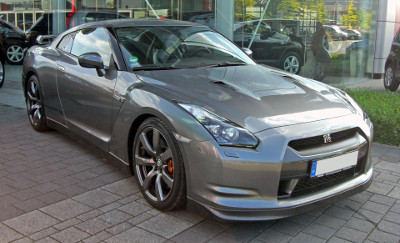
\includegraphics{Nissan.jpg}
\end{abstract}
\section{Samochód osobowy Nissan GT-R}
\subsection{Dostepne wersje}
\label{Dostepne Wersje}
\subsection{Jednostka Napędowa}
\label{Jednoska Napedowa}
\subsection{Skrzynia Biegów}
\label{Skrzynia Biegów}
\begin{table}
\ref{Dostepne Wersje}
-Nissan GT-R

-Nissan GT-R Gentleman edition


-Nissan GT-R Premium edition


-Nissan GT-R Black edition

-Nissan GT-R SpecV

-Nissan GT-R Track edition

-Nissan GT-R Egoist[4]

-Nissan GT-R Nismo

-Nissan GT-R Prestige Edition


\end{table}

\begin{table}
\ref{Jednoska Napedowa}
Jednostka Napędowa
\caption{Silnik} 
\begin{tabular}{c|c}
Pojemnosc & $3799$  \\
Konfig. & V6 DOHC biturbo \\
St. sprężenia & 9:1 \\
Zalecane paliwo & Benzyna 100 RON dopuszczalna 98RON \\
Napęd & Stały inteligentny 4x4
\end{tabular}

\end{table}
\begin{table}
\ref{Skrzynia Biegów} Skrzynia Biegów:
\begin{tabular}{c|c}

Typ przekładni & GR6 Dual Clutch \\
Przełożenie główne & 3,7:1 \\
Napęd & 4WD \\
\end{tabular}

\end{table}
\end{document}